% Options for packages loaded elsewhere
\PassOptionsToPackage{unicode}{hyperref}
\PassOptionsToPackage{hyphens}{url}
%
\documentclass[
]{article}
\usepackage{amsmath,amssymb}
\usepackage{iftex}
\ifPDFTeX
  \usepackage[T1]{fontenc}
  \usepackage[utf8]{inputenc}
  \usepackage{textcomp} % provide euro and other symbols
\else % if luatex or xetex
  \usepackage{unicode-math} % this also loads fontspec
  \defaultfontfeatures{Scale=MatchLowercase}
  \defaultfontfeatures[\rmfamily]{Ligatures=TeX,Scale=1}
\fi
\usepackage{lmodern}
\ifPDFTeX\else
  % xetex/luatex font selection
\fi
% Use upquote if available, for straight quotes in verbatim environments
\IfFileExists{upquote.sty}{\usepackage{upquote}}{}
\IfFileExists{microtype.sty}{% use microtype if available
  \usepackage[]{microtype}
  \UseMicrotypeSet[protrusion]{basicmath} % disable protrusion for tt fonts
}{}
\makeatletter
\@ifundefined{KOMAClassName}{% if non-KOMA class
  \IfFileExists{parskip.sty}{%
    \usepackage{parskip}
  }{% else
    \setlength{\parindent}{0pt}
    \setlength{\parskip}{6pt plus 2pt minus 1pt}}
}{% if KOMA class
  \KOMAoptions{parskip=half}}
\makeatother
\usepackage{xcolor}
\usepackage[margin=1in]{geometry}
\usepackage{graphicx}
\makeatletter
\def\maxwidth{\ifdim\Gin@nat@width>\linewidth\linewidth\else\Gin@nat@width\fi}
\def\maxheight{\ifdim\Gin@nat@height>\textheight\textheight\else\Gin@nat@height\fi}
\makeatother
% Scale images if necessary, so that they will not overflow the page
% margins by default, and it is still possible to overwrite the defaults
% using explicit options in \includegraphics[width, height, ...]{}
\setkeys{Gin}{width=\maxwidth,height=\maxheight,keepaspectratio}
% Set default figure placement to htbp
\makeatletter
\def\fps@figure{htbp}
\makeatother
\setlength{\emergencystretch}{3em} % prevent overfull lines
\providecommand{\tightlist}{%
  \setlength{\itemsep}{0pt}\setlength{\parskip}{0pt}}
\setcounter{secnumdepth}{-\maxdimen} % remove section numbering
% definitions for citeproc citations
\NewDocumentCommand\citeproctext{}{}
\NewDocumentCommand\citeproc{mm}{%
  \begingroup\def\citeproctext{#2}\cite{#1}\endgroup}
\makeatletter
 % allow citations to break across lines
 \let\@cite@ofmt\@firstofone
 % avoid brackets around text for \cite:
 \def\@biblabel#1{}
 \def\@cite#1#2{{#1\if@tempswa , #2\fi}}
\makeatother
\newlength{\cslhangindent}
\setlength{\cslhangindent}{1.5em}
\newlength{\csllabelwidth}
\setlength{\csllabelwidth}{3em}
\newenvironment{CSLReferences}[2] % #1 hanging-indent, #2 entry-spacing
 {\begin{list}{}{%
  \setlength{\itemindent}{0pt}
  \setlength{\leftmargin}{0pt}
  \setlength{\parsep}{0pt}
  % turn on hanging indent if param 1 is 1
  \ifodd #1
   \setlength{\leftmargin}{\cslhangindent}
   \setlength{\itemindent}{-1\cslhangindent}
  \fi
  % set entry spacing
  \setlength{\itemsep}{#2\baselineskip}}}
 {\end{list}}
\usepackage{calc}
\newcommand{\CSLBlock}[1]{\hfill\break\parbox[t]{\linewidth}{\strut\ignorespaces#1\strut}}
\newcommand{\CSLLeftMargin}[1]{\parbox[t]{\csllabelwidth}{\strut#1\strut}}
\newcommand{\CSLRightInline}[1]{\parbox[t]{\linewidth - \csllabelwidth}{\strut#1\strut}}
\newcommand{\CSLIndent}[1]{\hspace{\cslhangindent}#1}
\usepackage{booktabs}
\usepackage{longtable}
\usepackage{array}
\usepackage{multirow}
\usepackage{wrapfig}
\usepackage{float}
\usepackage{colortbl}
\usepackage{pdflscape}
\usepackage{tabu}
\usepackage{threeparttable}
\usepackage{threeparttablex}
\usepackage[normalem]{ulem}
\usepackage{makecell}
\usepackage{xcolor}
\ifLuaTeX
  \usepackage{selnolig}  % disable illegal ligatures
\fi
\usepackage{bookmark}
\IfFileExists{xurl.sty}{\usepackage{xurl}}{} % add URL line breaks if available
\urlstyle{same}
\hypersetup{
  pdftitle={STAT1378 Part I Report},
  pdfauthor={ADAB GILL},
  hidelinks,
  pdfcreator={LaTeX via pandoc}}

\title{STAT1378 Part I Report}
\author{ADAB GILL}
\date{}

\begin{document}
\maketitle

\section{Abstract}\label{abstract}

This report examines the relationships among height, weight, gender, and
physical activity levels within a sample dataset of men and women aged
26--45. The analysis utilizes linear regression, t-tests, and chi-square
tests to answer questions about linear relationships, mean differences,
and associations (\citeproc{ref-Xie2015}{Xie, Allaire, and Grolemund
2015}).

\section{Introduction}\label{introduction}

The study investigates three main questions: 1. Is there a linear
relationship between height and weight? 2. Does mean height differ
between males and females? 3. Is there an association between gender and
physical activity level?

Statistical methods like linear regression, t-tests, and chi-squared
tests are employed, aiming to answer these questions rigorously.

\section{Methods}\label{methods}

\subsection{Data Description}\label{data-description}

The dataset includes 1000 observations, each with the following
variables: - \textbf{ID}: Unique identifier for each participant. -
\textbf{Gender}: Male or Female. - \textbf{Height}: Participant height
in centimeters. - \textbf{Weight}: Participant weight in kilograms. -
\textbf{Physical Activity}: Level of physical activity (None, Moderate,
Intense).

\subsection{Statistical Tests}\label{statistical-tests}

\begin{itemize}
\tightlist
\item
  \textbf{Linear Regression}: To investigate the relationship between
  height and weight.
\item
  \textbf{t-Test}: To compare mean heights of males and females.
\item
  \textbf{Chi-squared Test}: To examine the association between gender
  and physical activity.
\end{itemize}

\section{Analysis and R Code}\label{analysis-and-r-code}

\subsection{Question 1: Linear Relationship between Height and
Weight}\label{question-1-linear-relationship-between-height-and-weight}

\begin{verbatim}
## 
## Call:
## lm(formula = weight ~ height, data = data)
## 
## Residuals:
##     Min      1Q  Median      3Q     Max 
## -35.701  -6.331   0.033   6.320  32.473 
## 
## Coefficients:
##              Estimate Std. Error t value Pr(>|t|)    
## (Intercept) -65.15096    7.75324  -8.403   <2e-16 ***
## height        0.77493    0.04471  17.334   <2e-16 ***
## ---
## Signif. codes:  0 '***' 0.001 '**' 0.01 '*' 0.05 '.' 0.1 ' ' 1
## 
## Residual standard error: 9.144 on 998 degrees of freedom
## Multiple R-squared:  0.2314, Adjusted R-squared:  0.2306 
## F-statistic: 300.5 on 1 and 998 DF,  p-value: < 2.2e-16
\end{verbatim}

\begin{table}
\centering
\caption{\label{tab:linear-model}Linear Regression Summary for Height and Weight}
\centering
\begin{tabular}[t]{lrrrr}
\toprule
  & Estimate & Std\_Error & t\_value & p\_value\\
\midrule
(Intercept) & -65.1509590 & 7.7532387 & -8.403064 & 0\\
height & 0.7749303 & 0.0447055 & 17.334135 & 0\\
\bottomrule
\end{tabular}
\end{table}

\begin{center}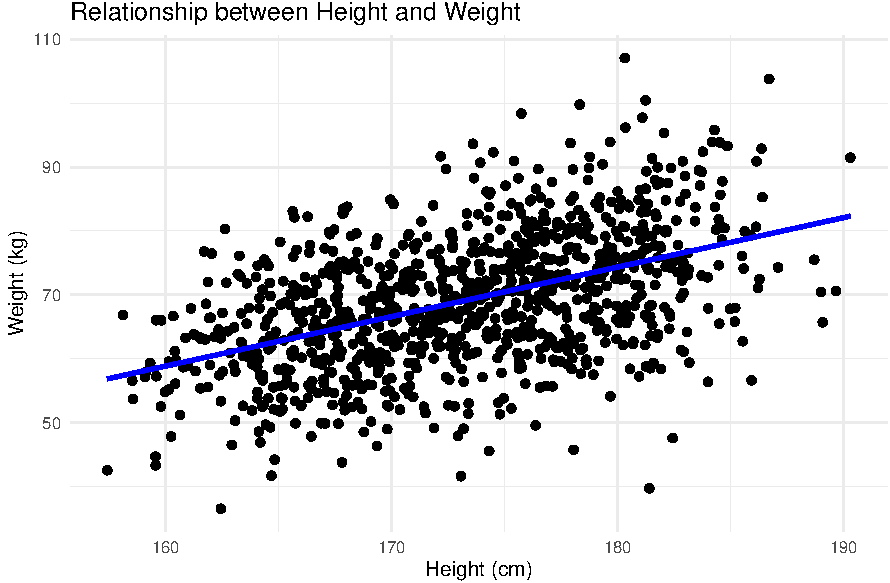
\includegraphics{PART-1_files/figure-latex/linear-model-1} \end{center}

\subsection{Results for Linear
Regression}\label{results-for-linear-regression}

Based on the linear regression analysis, a significant relationship was
found between height and weight, with a p-value of
\ensuremath{4.8071712\times 10^{-59}}. The slope of the line suggests
that with each centimeter increase in height, weight changes by
approximately 0.77 kg (\citeproc{ref-Moore2016}{Moore, McCabe, and Craig
2016}).

\subsection{Question 2: Difference in Mean Height between Males and
Females}\label{question-2-difference-in-mean-height-between-males-and-females}

\begin{longtable}[t]{lrrrlrr}
\caption{\label{tab:unnamed-chunk-3}t-Test Summary for Mean Height Comparison}\\
\toprule
 & Statistic & Parameter & p\_value & Confidence\_Interval & Mean\_Female & Mean\_Male\\
\midrule
t & -39.76867 & 978.8659 & 0 & -10.65 - -9.65 & 167.98 & 178.1299\\
\bottomrule
\end{longtable}

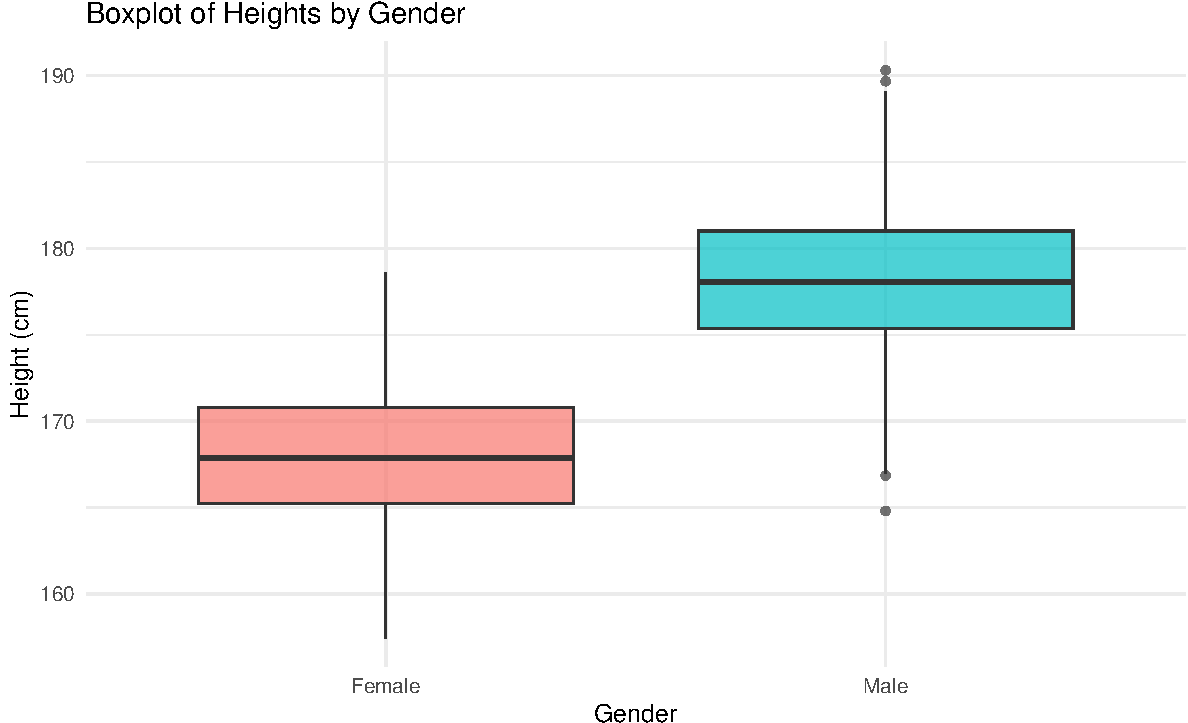
\includegraphics{PART-1_files/figure-latex/height-boxplot-density-1.pdf}

\subsection{Results for t-Test}\label{results-for-t-test}

The Welch Two Sample t-test shows a statistically significant difference
in mean height between males and females, with a t-value of -39.77 and a
p-value less than 2.2e-16. This result suggests that the mean height of
males (178.13 cm) is significantly greater than the mean height of
females (167.98 cm). The 95\% confidence interval for the difference in
means is between -10.65 and -9.65 cm, indicating that males are, on
average, taller than females in this sample. Since the p-value is much
smaller than 0.05, we reject the null hypothesis and conclude that there
is a statistically significant difference in height by gender. The
negative t-value and confidence interval (both in the negative range)
confirm that males are, on average, taller than females. The interval
provides an estimated range for the difference in means, reinforcing
that males are taller on average (\citeproc{ref-Agresti2018}{Agresti
2018}).

The hypotheses for the chi-squared test are:

\[
H_0: \text{Gender and Physical Activity Level are independent}
\]

\[
H_1: \text{Gender and Physical Activity Level are not independent}
\]

\subsection{Question 3: Association between Gender and Physical Activity
Level}\label{question-3-association-between-gender-and-physical-activity-level}

\begin{longtable}[t]{lrrr}
\caption{\label{tab:unnamed-chunk-4}Chi-Squared Test Summary for Gender and Physical Activity}\\
\toprule
 & Statistic & Degrees\_of\_Freedom & p\_value\\
\midrule
X-squared & 3.226111 & 2 & 0.1992778\\
\bottomrule
\end{longtable}

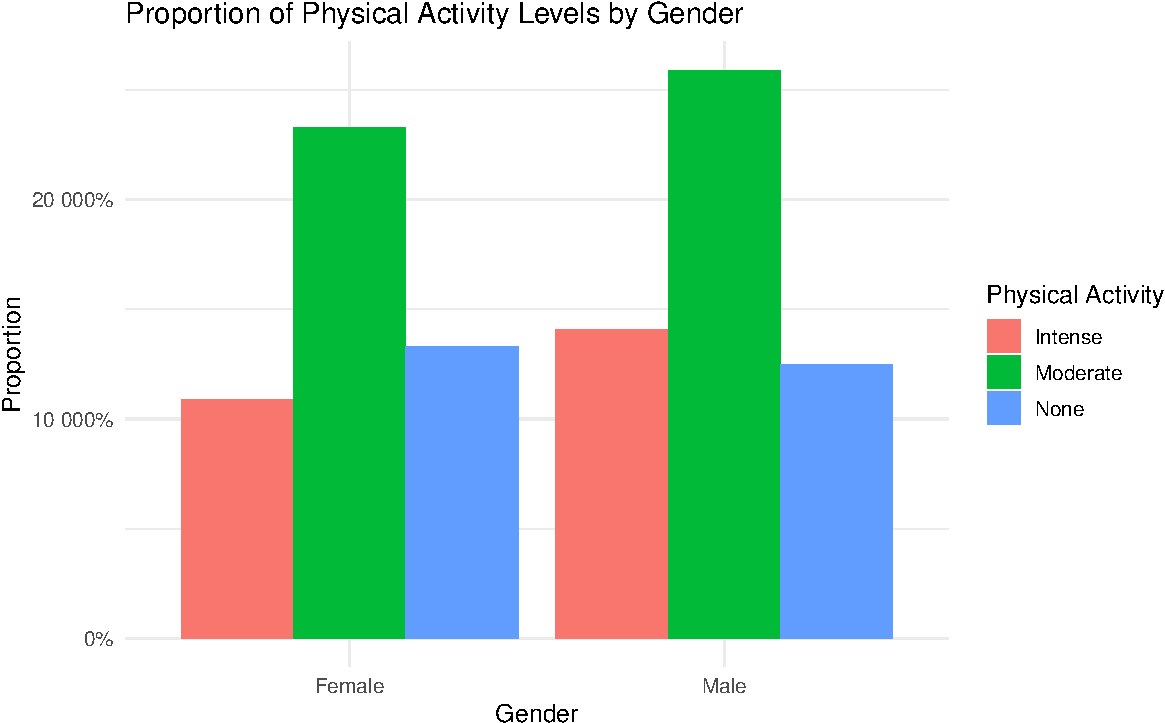
\includegraphics{PART-1_files/figure-latex/gender-activity-barplot-1.pdf}

\subsection{Results for Chi-squared
Test}\label{results-for-chi-squared-test}

The chi-squared test for association between gender and physical
activity level shows a chi-squared value of 3.23 with 2 degrees of
freedom and a p-value of 0.1993. Since the p-value is greater than 0.05,
we fail to reject the null hypothesis. This suggests that there is no
statistically significant association between gender and physical
activity level in this sample.

The p-value of 0.1993 is above the typical significance level of 0.05,
indicating that any observed differences in physical activity level by
gender are likely due to random chance. Failing to reject the null
hypothesis implies that gender does not have a significant association
with physical activity level in this data set.

\section{Conclusion}\label{conclusion}

\begin{enumerate}
\def\labelenumi{\arabic{enumi}.}
\item
  \textbf{Height and Weight Relationship}: The linear regression
  analysis indicates a statistically significant relationship between
  height and weight. This suggests that taller individuals in the sample
  tend to have higher weights, supporting a positive association between
  these two variables.
\item
  \textbf{Gender Differences in Height}: The t-test results show a
  statistically significant difference in mean height between males and
  females, with males being taller on average. This finding is
  consistent with general observations of height differences by gender.
\item
  \textbf{Gender and Physical Activity Level}: The chi-squared test for
  association between gender and physical activity level does not
  indicate a statistically significant relationship. This implies that,
  within this sample, physical activity levels do not differ
  significantly between males and females.
\end{enumerate}

\section*{References}\label{references}
\addcontentsline{toc}{section}{References}

\phantomsection\label{refs}
\begin{CSLReferences}{1}{0}
\bibitem[\citeproctext]{ref-Agresti2018}
Agresti, Alan. 2018. \emph{Statistical Methods for the Social Sciences}.
5th ed. Pearson.

\bibitem[\citeproctext]{ref-Moore2016}
Moore, David S., George P. McCabe, and Bruce A. Craig. 2016.
\emph{Introduction to the Practice of Statistics}. 9th ed. W.H. Freeman.
\url{https://www.macmillanlearning.com/college/us/product/Introduction-to-the-Practice-of-Statistics/p/1319013384}.

\bibitem[\citeproctext]{ref-Xie2015}
Xie, Yihui, J. J. Allaire, and Garrett Grolemund. 2015. \emph{R
Markdown: The Definitive Guide}. Chapman; Hall/CRC.
\url{https://bookdown.org/yihui/rmarkdown/}.

\bibitem[\citeproctext]{ref-Agresti2018}
Agresti, Alan. 2018. \emph{Statistical Methods for the Social Sciences}.
5th ed. Pearson.

\bibitem[\citeproctext]{ref-Moore2016}
Moore, David S., George P. McCabe, and Bruce A. Craig. 2016.
\emph{Introduction to the Practice of Statistics}. 9th ed. W.H. Freeman.
\url{https://www.macmillanlearning.com/college/us/product/Introduction-to-the-Practice-of-Statistics/p/1319013384}.

\bibitem[\citeproctext]{ref-Xie2015}
Xie, Yihui, J. J. Allaire, and Garrett Grolemund. 2015. \emph{R
Markdown: The Definitive Guide}. Chapman; Hall/CRC.
\url{https://bookdown.org/yihui/rmarkdown/}.

\end{CSLReferences}

\end{document}
